\chapter*{Introduction}
\addcontentsline{toc}{section}{\textit{Introduction}}
\markboth{\textit{Introduction}}{\textit{Introduction}}


\lettrine{\libertineInitialGlyph{T}}{here} is a satisfyingly simple general method for defining invariants of topological objects due to Thom, Arnold and Vassiliev. In broad strokes, the study of topological objects should take into account not only the objects, but also how they exist alongside their singular versions. The example of this thesis is that of topological knots: the space of immersions \(S^{1} \to \mathbb{R}^{3}\) contains knots (the embeddings), but also proper immersions that have one or more intersection points in \(\mathbb{R}^{3}\) and fail to be knots. The singular knots form a space of codimension one within the space of immersions; taking its complement divides the space of immersions into connected components which are exactly the knots. Similarly, inside the space of immersions with one or more intersection points lies the codimension one space of immersions with two or more intersection points, and it again divides up the space of one-singular-point immersions into connected components.

This continues, dividing the infinite-dimensional space of immersions into what is called the \textbf{stratification of the space of knots}. This includes the space of knots in the zeroth level of the strata, but it also includes all of the singular knots, and takes into account how the singular knots separate the space of knots. A rough schematic illustration of the strata might look like
\[
	\includegraphics[width=0.5\textwidth, valign=c]{graphics/stratification.pdf}
\]
but of course this two dimensional picture doesn't properly represent the infinite-dimensional stratification.

Vassiliev invariants are functions on the chambers of the strata (the knots) which take into account the walls of the strata by changing by a predictable amount across a wall (or higher dimensional stratum). This approach leads to a powerful analogy with polynomial functions, and a deep connection to Lie theory, as we will soon see.

\section*{Conventions}

All knots are assumed to be oriented and framed unless specified otherwise. Where a statement holds for a knot which is drawn unoriented, it holds for both orientations of that knot.
